% This is LLNCS.DOC the documentation file of
% the LaTeX2e class from Springer-Verlag
% for Lecture Notes in Computer Science, version 2.4
\documentclass[a4paper]{llncs}
\usepackage{makeidx}  % allows for indexgeneration
\usepackage{graphicx}
%
\begin{document}
%
%\frontmatter          % for the preliminaries
%
\pagestyle{headings}  % switches on printing of running heads
\addtocmark{Cloud Computing} % additional mark in the TOC
%
%\chapter*{Preface}
%
%TODO: ADD OWN PREFACE
%
%\tableofcontents
%
\mainmatter              % start of the contributions
%
\title{Service Level Checking - Ensuring Service Level Agreement Compliance in Cloud Computing}
%
\titlerunning{Cloud Computing}  % abbreviated title (for running head)
%                                     also used for the TOC unless
%                                     \toctitle is used
%
\author{Hubert~Hirsch \and Frieder~Ulm \and
Philipp~Raich}
%
\authorrunning{Hubert Hirsch et al.} % abbreviated author list (for running head)
%
%%%% list of authors for the TOC (use if author list has to be modified)
\tocauthor{Hubert Hirsch, Frieder Ulm, and Philipp Raich}
%
\institute{Distributed Systems Group, TU Wien, 1040 Wien, Austria,\\
\email{e0625008@student.tuwien.ac.at},
\email{e0527031@student.tuwien.ac.at},
\email{philipp.raich@student.tuwien.ac.at},\\
 home page: \texttt{http://www.infosys.tuwien.ac.at/}}

\maketitle              % typeset the title of the contribution

\abstract{
In Cloud Computing, \textit{Service Level Checking} (SLC) is the verification of compliance with negotiated \textit{Service Level Agreements}\\(SLAs) with a cloud computing provider. The virtualization layer inherent to the cloud computing model makes it is more complex to monitor cloud usage and to anticipate and prevent SLA violations. Energy efficiency is becoming an increasingly important factor, placing weight on the importance of cloud optimization. After a brief introduction about cloud computing and the current state of affairs, we will describe the necessary tasks involved in SLC and the benefits to both cloud providers and customers when SLC is performed directly by the cloud provider in his own cloud. SLC as a process is described with the help of the \textit{MAPE loop}. This paper aims at giving the reader a solid understanding of the importance of Service Level Checking, the state of the art techniques and their implications regarding energy efficiency, as well as emerging fields of research.
}

\section{Introduction}
Cloud computing is a topic of ever-increasing importance. Before clouds, grid computing was the technology of choice. However, as can be seen in Fig.~\ref{fig:rise_cloud}, cloud computing has surpassed grid computing in Google trends since 2007, and the upward trend seems to continue~\cite{Alhamad11}.

\begin{figure}[Ht]
	\centering
		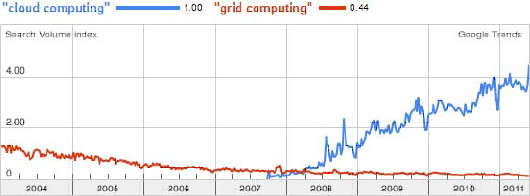
\includegraphics[width=0.6\textwidth]{figs/rise_cloud.png}
	\caption{The Rise of Cloud Computing, taken from~\cite{Alhamad11}}
	\label{fig:rise_cloud}
\end{figure}

Cloud computing allows end-users for custom tailored online storage and server solutions using virtualization combined with grid technologies. In contrast to traditional web hosting with a fixed bandwidth, storage and pre-installed software suite, e.g. an HTTP Server with PHP5, cloud computing provides \textit{IaaS} (Infrastructure as a service), \textit{PaaS} (Platform as a Service) or \textit{SaaS} (Software as a Service).\\
IaaS for example, gives a user access to a (typically virtual) remote machine with agreed upon system hardware specifications, where on the provider’s side, various machines participate in providing this service transparently to the user. PaaS includes a preinstalled operating system and certain tools as platform available to the user, where SaaS is the most similar to the classical web server, which it gives the user access to a service via a cloud software similarly to software installed on the own computer, but with the mentioned transparent elasticity provided in the background by the cloud provider. Amazon’s EC2 cloud, as an example, gives the user the choice to select from different attributes, e.g. operating systems or software installed (PaaS and Saas) but also allows the installation of own operating system images on the virtual machine instance available to the user (IaaS)~\cite{Graubner}.\\
Furthermore the involved parties must agree on latency, bandwidth and other common network characteristics met by the provider of the service. The user can then set up his machine with the necessary software to run his web application, game server, et cetera; with growth of the user base, additional demands in regards to scalability can be met by purchasing additional resources.\\
The agreements between the host and the user of the service is recorded in the \textit{Service Level Agreements} (SLAs) and typically contains contractual agreements, as well as the host of requirements common to all web based programs (bandwidth, response time, et cetera) also known as \textit{Quality of Service}(QoS)-parameters, usually formalized as \textit{Service Level Specification} (SLS) as part of the SLAs. For the user of a service it is most important that he can rely on the fulfillment of these constraints~\cite{Undheim11}.\\

The provider on his end, tries to \textit{minimize his resource consumption} (in respect to e.g. used energy or incurred costs) by different techniques, as e.g. smartly distributing virtual machines over the available physical hardware, reducing available resources on virtual machines currently experiencing low loads, passivating virtual machines that are currently idle, and so on.\\
On the other hand, aggressive optimization might be problematic, e.g. a passivated virtual machine will experience a delay upon an incoming request due to the need for (re-)activation. The more aggressive the provider tries to minimize his resource consumption, the more likely he will \textit{violate an SLA} with one of his customers.\\

Does a occurring situational delay constitute a breach of the minimum response time specified in the SLA? In addition, who is responsible for monitoring and raising a red flag upon such violations? Also taking into consideration the issues of proof and trust in a business agreement, the matter becomes complicated and gains importance for both, the provider and the user of a service.\\

This paper tries to give an \textit{overview over the state of the art techniques}, which have been proposed so far, meant for the cloud provider to be undertaken if he wishes to monitor its system and proactively prevent, or reactively correct, SLA violations.\\

\section{Service Level Checking}
Due to the fact that cloud computing as a largely commercially successful technology has only started emerging from 2006 on, the primary focus of development was to provide a working infrastructure. Now that cloud computing has established itself on the market (and in fact as a market itself), verifying SLA compliance is becoming a more viable field of research~\cite{Emeakaroha10a}.\\
In light of the existing competition that the major providers are facing, SLC is a desirable feature to offer to customers. The mainstream approach so far, was to shift the responsibility of verifying SLAs to the customer. As a result a market for cloud monitoring providers has emerged. These try to verify SLA compliance for the customer and provide evidence in case of violations, in addition they \textit{monitor usage} in order to prevent bad surprises at the end of the month when confronted with the bill.\\

While this practice works up to a degree, performing Service Level Checking directly within the provider’s infrastructure has several benefits. If a customer decides to enter a contract with a specific cloud provider, it makes more sense for him to purchase the corresponding SLC services from the same provider rather than having to deal with a third party.\\

From the providers perspective, due to direct access to all soft- and hardware, no one is better able to monitor the cloud in detail, than the provider himself. Better analysis and understanding of the own cloud in turn allows for better optimizations, thus reduced costs and/or a even more competitive offering in respect to better conditions for the customer and allows the provider to distinguish himself from the competition. Due to increased awareness in the public, especially \textit{energy efficiency} in clouds and thus their energy aware providers are better perceived by the public and so are all of their services.\\
Finally, seeing as cloud monitoring/SLC is an emerging business, leaving the field to other companies means forfeiting potential revenues.\\

It should also be noted, that it is not enough for a cloud provider to take on the responsibility of performing SLC. Even the most reputable provider will be faced with \textit{issues of trust} when money is involved. Alleviating the need for a third party company that performs service level checking, at the same time raises the requirement for a different trusted third party, to verify the truthfulness of the cloud provider.\\

\section{Achieving SLC}
\label{sec:achieving_slc}
\subsection{Identifying Information}
The top down approach the cloud provider can apply, is to identify the high level information that one wants to
\begin{enumerate}
	\item make accessible to the user,
	\item is required for optimization for his own teams and
	\item needed to compare against the SLAs.
\end{enumerate}

From there, one can identify the lower tier information needed to compile the desired high level information.\\

Bottom up, a list of easy to obtain low level information can be created. This low level metrics can then be analyzed for possible high level information to be derived.
Although this sounds simple and straightforward, it is actually a complex task because of various interdependencies between the many low level metrics, and depends largely on the implemented architecture~\cite{Undheim11}. Furthermore, the resulting functions need not to be simple one to one mappings and may have difficult to predict results.\\

Although cloud providers tend to introduce their own notion of established high level metric identifiers, they will be largely comparable across different cloud providers, due to the abstractions implied by the user requirements. The biggest differences are expected to be found in the exact composition of low level data, due to the different ways in which providers implement their clouds. With high probability, there will be differences in the exact way that similar or comparable SLA parameters are interpreted in different cloud infrastructure implementations. \textit{Availability} for example can be derived from any combination of downtime, bandwidth shortfalls, high latency periods, et cetera. \\
Because no standard for the interpretation of common SLA parameters exists, SLA definitions move away from exact quantification of values and instead attempt to define the user experience in more verbal terms~\cite{Roxburgh11}.

\subsection{Processing Information}
Subsequently the gathered data has to be processed in some way to provide new insights into the system. The extracted information can be analyzed for short term benefit, such as noticing impending SLA violations. A large host of accumulated data over a period of time can also give statistical information about the system for a long term benefit, e.g. to adjust a time-of-the-day rulebase or to improve an employed algorithm and their parameters.\\

\subsection{Using Information}
Ultimately the obtained knowledge can be used to make \textit{beneficial changes} to the own system, make short term decisions in regard to resource allocation and be made available to users as part of the provided service. When provided with detailed usage statistics, customers themselves can draw their own conclusions from their individual usage sand optimize their workflow.

\section{Cloud Architecture}
Due to the different constraints that SLAs entail, as well as the dynamic nature of incoming requests, it is no longer possible to utilize traditional system-centric resource management architecture. Instead, to ensure SLA compliance, it is necessary to regulate the cloud based on supply and demand of the cloud’s resources. To do this, a common high-level cloud architecture has emerged. This architecture consists the following components~\cite{Buyya09}:
\begin{itemize}
	\item Cloud management component: The cloud manager component is responsible of managing the cloud. Within the cloud manager, several  sub-components exist:
	\begin{itemize}
		\item VM monitor: The VM monitor keeps track of currently allocated virtual machines, their resource usage, as well as their overall reserved resources. The VM monitor can also dynamically create new virtual machines to respond to new service request requirements, or destroy allocated virtual machines to free resources. Furthermore, the VM monitor has an overview of physical machine resources and manages these as necessary.
		\item Dispatcher: The dispatcher deploys incoming application requests on a virtual machine environment. If no suitable virtual machine exists, it interacts with the VM monitor in order to have one created.
		\item Service Request Monitor: The Service Request monitor tracks dispatched service requests; it supplies information regarding currently executing applications such as execution progress and resource usage.
		\item Service Request Examiner and Admission Control: This component provides an interface to users to submit applications to the cloud manager. Before the application is accepted or rejected it is interpreted for service level objective requirements. It decides if enough resources are available to execute the incoming application. To make these decisions, it needs to interact with the VM monitor and service request monitor components.
		\end{itemize}
	\item Physical Machine: Physical machines are essentially computing servers that provide resources to the cloud. The computers that make up the computing infrastructure of the cloud need not necessarily be homogeneous.
	\item Virtual Machine: To meet accepted service requests, physical machines are sliced into virtual machines that each run their own operating system. These virtual machines are then collected into pools based on the resources they have and managed by the VM monitor. Virtual machines can be created and assigned to a resource pool dynamically as demand on that pool rises. They can then be destroyed when they are no longer required. The ability to provision and destroy virtual machines on the fly allows a vendor to provide Infrastructure as a Service (IaaS).\\
	\end{itemize}

\section{SLC Approaches}
The steps described in section~\ref{sec:achieving_slc} will always be necessary in some way or another. Because of this, the idea for a unified pattern suggests itself. This task is not trivial because of the differences between the proprietary cloud implementations and lack of standards.\\

An already well proven approach that seems to fit the task of SLC is the \textit{MAPE loop}.\\
This part of the paper will give a short introduction into the MAPE loop and further use it to demonstrate the different concepts and methods which can be used to realize SLC, as most proposed approaches can be seen as implementing variants of it to achieve the aforementioned goals and thus can be broken down into their respective MAPE-steps.\\
The focus lies on the described practices. The MAPE loop (being a well known pattern) is used as an abstraction/categorization of the described practices and how they work together structurally.

\subsection{MAPE Loop}
The MAPE loop is a common abstract approach for controlling a autonomous system acting upon a (complex) environment. It is taken from artificial intelligence processing and it describes a system that only needs sporadic/no user input and otherwise perceives its environment, analyzes its, updates itself and infers actions to take. The MAPE approach is an iterative loop that breaks this (for machine intelligence) complex task down to these abstract consecutive steps: \textit{Monitor, Analyze, Plan and Execute} (see Fig.~\ref{fig:mape}).\\
Consequently, during the \textit{Monitor} step, the environment (or its relevant abstraction metrics) is perceived, during the \textit{Analyze} step the gathered information is broken down to relevant conclusions that conclude in a plan formed during the respective \textit{Plan} step which is executed (mostly acting on the perceived environment) in the \textit{Execute} step.\\

\begin{figure}[Ht]
	\centering
		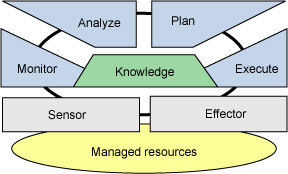
\includegraphics[width=0.6\textwidth]{figs/mape.png}
	\caption{The MAPE-Loop}
	\label{fig:mape}
\end{figure}

Additions to the original MAPE loop exist: elements of \textit{knowledge management} and \textit{semantic web} development can influence the autonomous behaviour of the system after deployment and during execution in the environment.\\
Simple MAPE systems without knowledge bases try to use static rules to choose actions from, whereas an enhanced MAPE loop acting upon a knowledge base (MAPE-K) learns from the perceived environment during its lifetime and tries to use this information to deal with new information gathered (see Fig.~\ref{fig:mape})\\
Furthermore, an adaptation phase can be added to the loop to help do all the steps necessary before the start of an application, e.g. adjust the cloud infrastructure as well as the applications that are to be deployed on it with special regards to fulfill the monitoring requirements (see section~\ref{sec:adaption})\cite{Maurer11}.\\
\textit{Case-Based Reasoning} (CBR) can be utilized to improve scheduling algorithms contained in the knowledge base. By using CBR, the MAPE loop helps to avoid future SLA violations by intelligently scheduling applications based on the up to date monitored metric values and comparable situations perceived in the past~\cite{Maurer10}\cite{Maurer11}\\
Under certain frameworks the analyzing and planning phase are cumulated into one single step  because of their highly linked nature, e.g. all frameworks embedded into the \textit{Foundations of Self-Governing ICT Infrastructure} (FoSII)~\cite{Maurer11}\cite{Emeakaroha10a}\cite{Emeakaroha10b}.

\subsection{Sensors and Effectors}
From an abstract perspective, a MAPE system perceives its environment by using appropriate sensors. Sensors in this context are the sum of information gathering devices, which can be physical sensors located e.g. on the motherboard of the according computer measuring the physical performance parameters such as heat output, energy consumption, voltages, current flow, et cetera.\\
Other machine specific sensory data can be retrieved from monitoring software providing (in this context even more important) information pertaining to resource usage attributes such as used storage, CPU load, memory load, et cetera.\\
Finally other sensors (e.g. integrated into attached network devices) can give detailed information in regards to network throughput, latency, network load, lost packets and so on that can be used to gain information about the state of one machine or a group of machines~\cite{Gunter00}.\\

The challenge here is to gather the different sensory inputs at short notice, as new information may lead to an immediate action necessary. Some of the sensors can be easily queried using SNMP (Simple Network Management Protocol), others will require custom tailored solutions or integration of proprietary APIs specific to the hardware devices.\\
Further it is possible to add an additional communication infrastructure to gather this information, to avoid the queried sensory communication being interrupted by application-specific communication, or vice versa.\\

Effectors can be realized as calls to control interfaces of the cloud manager, or if necessary, as a call to any of the control-interfaces of the lower-level entities, e.g. a virtual machine.\\

Finally, the constraints (i.e. the service level objectives) which are to be met by the loop itself and thus act as the control value input to the loop are (or may be derived of) the user requirements, i.e. the SLAs.

\subsection{Adaptation}
\label{sec:adaption}
The adaptation step is invoked whenever a new application enters the cloud managed state. It consists of SLA contract establishment, initialization of the monitoring systems for the new application, and matching of private to public provider and consumer templates. A mismatch of said templates would be different units of measurement for an attribute. An automated mechanism to resolve these differences is necessary and often own modules are installed to handle the related tasks transparently for the customer and the cloud manager~\cite{Freitas10}. Missing and mismatching attributes can either be handled by the system itself, or third party providers prompted for information regarding certain attributes~\cite{Maurer11}. 

\subsection{Monitor}
The monitoring component of the loop utilizes the available sensors to keep track of the system’s current status. For this purpose various tools are available, for example ganglia~\cite{Massie04}. To be able to utilize the measured values, the various low level metrics have to be \textit{compiled into high level metrics} that can be compared to service level objectives, or made available to the user~\cite{Maurer11}. This feature is usually not provided by the tools for monitoring low level metrics and hence must be implemented by a higher level framework.\\

Simple high level metrics can be mapped directly to low level metrics. More often, however, it is necessary to aggregate different low level metrics in order to map them to an SLA parameter. One example is \textit{Availability} as high level metric, which can be broken down into uptime and downtime as low level metrics. To correlate the two, a formula as seen in Fig.~\ref{fig:lo2hi} can be utilized.\\

\begin{figure}[Ht]
	\centering
		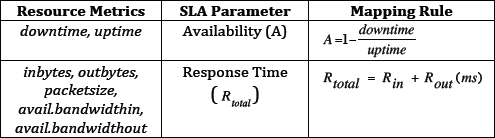
\includegraphics[width=0.8\textwidth]{figs/lo2hi.jpg}
	\caption{A Sample of Low-Level Metrics to High-Level Metrics Mappings}
	\label{fig:lo2hi}
\end{figure}

For MAPE-K Loops, during the monitoring stages, the knowledge base is updated to keep track of the newly measured metrics to reflect how the system has changed and performs over time. As such, the learning agent’s ability to forecast the state of the environment is improved with each iteration of the monitor component of the MAPE cycle.

\subsection{Analyze}
During the analyzation phase, the information gained from the monitor is processed against the system rule database to determine the current system status. One way to do this is to use statically defined rules, e.g. specified threat threshold. These act as early warning boundaries indicating that values indicate an an approaching breach of an SLA objective. By using this technique, gathered values can be compared and applied to rules without complex calculations~\cite{Freitas10}. The rules might as well be more sophisticated, naturally.
When a MAPE-K loop is used, rules may be used to dynamically adjust thresholds based on the system status ~\cite{Emeakaroha10a}.\\

Another way to classify the current system state is to use models. Models are used to abstract the system state in a way that makes it easier to comprehend and work with. Multiple models can be used to match various system states~\cite{Shao10}.\\

Models, like thresholds, can also be adjusted. Application behavior observed over a span of time can be used to adjust the provisioning of resources for an application. Taking this idea further, the time span can be increased to several days/weeks/months. Such data can be gathered on a per-application basis, or inferred from similar applications. Anticipating the resource needs of an application allow the host to allocate the required resources in advance, rather than during load times.\\

Fig.~\ref{fig:usage} shows a real life example of load distribution on a cloud during the day as average over one month. The analytical insight gained from this particular statistic would allow the cloud’s host to distribute the VMs in his cloud before 2pm. This would reduce the necessary amount of VM migrations along physical machines.\\

\begin{figure}[Ht]
	\centering
		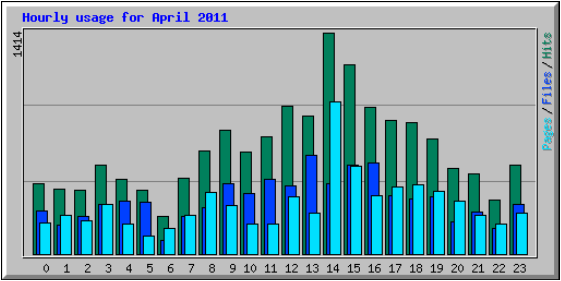
\includegraphics[width=0.8\textwidth]{figs/usage.png}
	\caption{A Sample Usage Statistic for a typical Cloud Application over one Month}
	\label{fig:usage}
\end{figure}
 
The analyze phase might be consolidated with the following plan phase in some frameworks, due to their closely related functionality.

\subsection{Plan}
In the planning step the findings of the analysis are used as a base for the planner to choose a set of possible actions to perform. The planner can be used to work towards possibly contradictory paradigms, such as performance or energy efficiency. It is important to settle on a common ground that is applicable for the purpose of the application, fulfills its service level objectives, and the cloud provider’s policy.\\

Intuitively, an application would be provisioned with as many resources as required and no more; however, it is imaginable to provide more resources to the application than agreed on in the SLA. This practice would make sense if the cloud still has unallocated resources which could be used by the application when needed. While passing up savings in energy costs, the additional service provided to the user could give the cloud operator a competitive edge in the market.\\

The simplest approach to determining which action to take is a simple and static rule-set database. Rule-sets are statically defined to cover the entire domain of possible states the system can be in, and the respective actions to execute. Already implemented platforms such as \textsc{Drools}~\cite{Drools} may be used to realize the rule-based approach.\\

If a \textit{MAPE-K loop} is used, the rule base can be expanded dynamically with case based reasoning, inferring new actions from similar cases that occurred in the past~\cite{Maurer10}. This method tries to match the current system state against a case that contains:
\begin{itemize}
	\item a previously encountered similar state
	\item actions executed to improve it and
	\item the resulting positive/negative effects.
\end{itemize}

The system can then try to improve already good results, finding an optimum, or avoid repeating mistakes.\\

Alternatively an \textit{algorithmic approach} is possible, where heuristic optimization techniques for \textit{Multi Dimensional Bin Packing} (MDBP) (as a multitude of attributes must be considered) may be utilized to produce alternative assignments of the one currently present in the cloud, by primarily optimizing usage of available resources~\cite{Feller11}. Hence the primary goal of this approach is to drastically reduce (energy) costs for the provider by transforming it into an \textit{optimization or approximation problem}.\\
Not only in the end, but also during execution of the algorithm, each (preliminary) assignment produced by the algorithm needs to be evaluated under a rating function that must not simply choose the assignment that reduces overall costs at any price, as the resulting assignment still should be able to handle possible spontaneous load increases and thus needs to provide standby resources.\\
Furthermore, an optimal assignment may be useless, if it cannot be applied to the cloud at all or in reasonable time and with reasonable costs generated by the move between the actual and the new assignment.\\
Hence, as this approach may elegantly solve the problem of optimization, other significant problems adhere to it and must be solved before it can be applied. Although various solutions are thinkable (e.g. rule-based rating function, complex assignment and moving constraints), the authors were not able to find a concrete proposal for the solution to this problem.\\

As already mentioned before, the plan phase and the aforementioned analyze phase might be consolidated into one step in some frameworks, due to their closely related functionality.

\subsection{Execute}
During the execution phase, the cloud manager attempts to execute the actions of the selected plan. For this to be possible, the executing module must be able to call the according methods through appropriate interfaces, so that the changes to the cloud take place as intented by the planning phase. Usually, the executor must be aware of the capabilites of the responsible cloud manager and its (hopefully standardized) interface~\cite{Freitas10}.
Some typical actions in cloud are:

\paragraph{Virtual Machine Migration}, VM migration describes the practice of moving a snapshot of a VM from one physical machine to another, preserving its state. This action becomes necessary when a single physical machine can no longer host the load required by its VMs or is expected not to be able to do so in the near future. In any case, this procedure always takes a certain amount of processing and transmission time. The costly nature of migrating VMs raises the need for efficient planning algorithms~\cite{Zhao09}.

\paragraph{Application Migration}, The migration of an entire virtual machine is relatively costly. It is associated with a temporary interruption of the service level and comes with overhead due to the computational power, storage, bandwidth, etc. required to migrate the machine. Application migration follows the same idea as VM migration. The image of an application running on a virtual machine is transferred to a different VM. The benefit is that only the application itself has to be transferred instead of the entire VM image. This can be done for simple applications, however it becomes less feasible the deeper an application is integrated with its environment, e.g. a distributed application which spans multiple virtual machines or depends on other applications on the same virtual machine.

\paragraph{Passivating Physical Machines}, After heavy load phases the cloud can end up in a state where the physical machines are running few VMs, being underutilized. The cloud manager will then likely migrate virtual machines, redistributing them to achieve higher utilization of each machine. The goal is to free any number of physical machines, so that they can then be passivated to save costs.

\paragraph{Passivating Virtual Machines}, One possibility worth consideration, in specific cases like SaaS, HTTP servers, etc. is to passivate an idle virtual machine, the applications of which are blocking while waiting for input. This could be beneficial if the overhead of running the VM compared to the hosted applications is too big and a lot of such VMs are running inside the cloud.\\

Executing any kind of action will have an effect on the knowledge base, influencing future iterations of the MAPE cycle. Before a plan can be put into practice, it is necessary to check whether it is still possible to do so; the system status may have changed between the planning and execution phase, rendering some plans infeasible.\\

The specific details of the execution phase will be inherent to their respective cloud infrastructure implementations. Ultimately, only owners of a cloud infrastructure will be able to test the practical realizations proposed in various papers.\\
Researchers, however, are limited to simulating the real world in virtual or significantly smaller lab environments. As a result, the insight gained from their predictions is not completely accurate; side effects occurring in a real cloud environment are hard to anticipate and take into account.

\subsection{Other Approaches}
One possible other approach is the \textit{top down approach} presented in~\cite{Nguyen09}. It divides the problem into two Layers: a \textit{Local Cecision Module} (LDM) and a \textit{Global Decision Module} (GDM). A LDM acts upon the application environment itself and the associated virtual machines and is responsible for the adherence to the service-level objectives defined for this application. For this purpose the LDM obviously needs an application-specific performance model, which unfortunately is not presented by the authors.\\
The sum of all LDMs interact with a GDM on every control loop cycle, which itself incorporates the main decision-making entity. The GDM perceives a LDM as black-box and only receives the LDMs utility function and on the other side the system-level performance metrics from all virtual and physical machines. As a result the GDM conducts the cloud hypervisor, so the current state of the cloud may be improved or repaired, and sends appropriate notifications to the LDMs afterwards.\\
One big drawback of the approach, is the lack of overview over the cloud in the decision-making entity, the GDM, as it has only an \textit{abstract view of the applications and their VMs}. This implies that it will most certainly have diminished possibilities in respect to optimization of the current cloud state.\\

\section{Emerging Research}

\subsection{Effective Virtual Machine Migration}

Energy costs account for a substantial amount of a data centers total cost. In order to save energy it is desirable to distribute the current load over as few physical machines as possible. Because of the dynamic nature of a cloud, the resource needs of an application/virtual machine can increase or decrease sporadically. As a result, the VM may require migration to a different physical machine. This physical machine can even be located in a different network altogether. Efficient distribution of virtual machines allows the cloud manager to passivate or shut down idle physical machines, reducing the energy footprint of the cloud~\cite{Graubner}.\\

For the applications running on the virtual machine this transition should not be noticeable. Any interruption of service associated with the migration itself constitutes a potential breach of the SLA. This makes methods which allow the migration of a VM without or with minimal service interruptions and downtime, like the Eucalyptus framework, an interesting topic of research~\cite{Zhao09}. A complementary measure/alternative, would be to anticipate the need for migration before it becomes absolutely necessary.\\
Anticipating the need for migration also allows the provider to use more naive migration methods, rather than resource hungry mechanisms like, for example, preparing a copy of the VM on another physical machine while the original VM is still active.

\subsection{3-Tier Cloud Monitor Architecture}
This pattern is a proposal for a divide and conquer approach to manage the complexity of monitoring data from the various sources within a cloud. It uses a component based architecture for the implementation of the monitor system using a 3-tier architecture.
A seen in Fig.~\ref{fig:3tier_monitor}, the low level core monitor is situated at the lowest data collection point, gathering the available raw system metrics, and aggregates them into low-level indicators. These are sent to the data collector  which aggregates them to high level metrics and passes them on to the service monitor, which aggregates the received data and finally matches it against the service level objectives~\cite{Chazalet10}.\\

\begin{figure}[Ht]
	\centering
		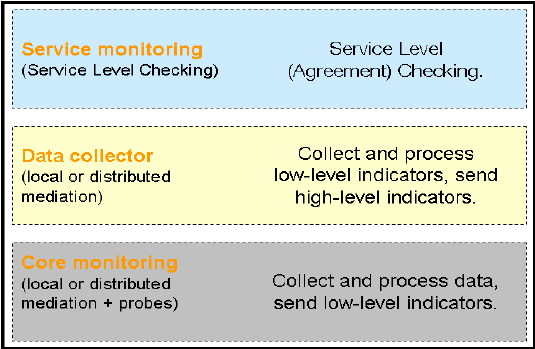
\includegraphics[width=0.6\textwidth]{figs/3tier_monitor.png}
	\caption{The Architecture of the 3tiered Monitor, taken from~\cite{Chazalet10}}
	\label{fig:3tier_monitor}
\end{figure}

The architecture is rather basic, it constitutes a pure monitoring approach which does not introduce any corrective measures to the system, instead checks for violations exclusively. The target user of this architecture would be a third party monitoring a cloud. At the lowest level of this monitor requires “probes” which gather available data from the cloud. This data has to either be made available by the cloud provider through services or implicitly derived through use of the cloud. Again there is an issue of trust when the data for the probes is provided directly by the cloud provider for third party monitoring.

\section{Conclusion}
Service level checking provides obvious benefits to the cloud provider: Additional service is provided to the customer by allowing insight into detailed usage statistics and avoiding SLA violations. The provider gains a better understanding of the cloud, leading to improvements of the cloud manager, resulting in more efficient clouds.\\

The distributed nature of clouds, virtualisation and heterogeneous cloud implementations are an obstacle in developing frameworks and patterns. Adapter interfaces tying the cloud to the proposed frameworks exhibit a high degree of complexity. The decisions involved in developing an action plan to react to different cloud states potentially vary in numerous aspects, as do the details of executing plan actions on the cloud. Well defined frameworks that can be applied to the various clouds are important.\\

Architectural patterns such as the 3-tier cloud monitor architecture help reduce the complexity of implementing and maintaining the monitoring component of a cloud manager. Applying the A-MAPE-K loop to cloud computing, is one possible way of consolidating the required actions in one pattern.\\

High energy costs and the growth rate of computational requirements make it important for cloud providers to increase the cloud’s utilization, by employing smart optimization techniques to increase efficiency. Forecasting, VM migration and passivation are some of the possible ways to lower costs associated with running a cloud. By monitoring service level objectives and employing service level checking, future behaviour of deployed and incoming applications can be anticipated and SLA violations avoided. However, methods for mapping high-level service level objectives to low-level gathered sensory data is far from trivial.

% ---- Bibliography ----
%
\begin{thebibliography}{[MT1]}

\bibitem{Alhamad11}
Alhamad, M.; Dillon, T.; Chang, E.; ,
"Service Level Agreement for Distribued Services: A Review",
Dependable, Autonomic and Secure Computing (DASC), 2011 IEEE Ninth International Conference on , vol., no., pp.1051-1054, 12-14 Dec. 2011

\bibitem{Graubner}
Graubner, P.; Schmidt, M.; Freisleben, B.; ,
"Energy-efficient Virtual Machine Consolidation for Cloud Computing," IT Professional , vol.PP, no.99, pp.1, 0

\bibitem{Undheim11}
Undheim, A.; Chilwan, A.; Heegaard, P.; ,
"Differentiated Availability in Cloud Computing SLAs," Grid Computing (GRID), 2011 12th IEEE/ACM International Conference on , vol., no., pp.129-136, 21-23 Sept. 2011

\bibitem{Emeakaroha10a}
Emeakaroha, V.; Calheiros, R.; Netto, M.; Brandic, I.; Rose, C.; ,
"DeSVi: An Architecture for Detecting SLA Violations in Cloud Computing Infrastructures" given at the 2nd International ICST Conference on Cloud Computing (CloudComp 2010) Barcelona, Spain October 25 - 28, 2010.

\bibitem{Roxburgh11}
Roxburgh, D.; Spaven, D.; Gallen, C.; ,
"Monitoring as an SLA-oriented consumable service for SaaS assurance: A prototype," Integrated Network Management (IM), 2011 IFIP/IEEE International Symposium on , vol., no., pp.925-939, 23-27 May 2011

\bibitem{Maurer10}
Maurer, M.; Brandic, I.; Emeakaroha, V.C.; Dustdar, S.; ,
"Towards Knowledge Management in Self-Adaptable Clouds," Services (SERVICES-1), 2010 6th World Congress on , vol., no., pp.527-534, 5-10 July 2010

\bibitem{Buyya09}
Buyya, R.; ,
"Market-Oriented Cloud Computing: Vision, Hype, and Reality of Delivering Computing as the 5th Utility," Cluster Computing and the Grid, 2009. CCGRID '09. 9th IEEE/ACM International Symposium on , vol., no., pp.1, 18-21 May 2009

\bibitem{Maurer11}
Maurer, M.; Breskovic, I.; Emeakaroha, V.C.; Brandic, I.; ,
"Revealing the MAPE loop for the autonomic management of Cloud infrastructures," Computers and Communications (ISCC), 2011 IEEE Symposium on , vol., no., pp.147-152, June 28 2011-July 1 2011

\bibitem{Emeakaroha10b}
Emeakaroha, Vincent C.; Brandic, Ivona; Maurer, Michael; Dustdar, Schahram; ,
"Low level Metrics to High level SLAs - LoM2HiS framework: Bridging the gap between monitored metrics and SLA parameters in cloud environments," High Performance Computing and Simulation (HPCS), 2010 International Conference on , vol., no., pp.48-54, June 28 2010-July 2 2010

\bibitem{Gunter00}
Gunter, D.; Tierney, B.; Crowley, B.; Holding, M.; Lee, J.; ,
"NetLogger: a toolkit for distributed system performance analysis ," Modeling, Analysis and Simulation of Computer and Telecommunication Systems, 2000. Proceedings. 8th International Symposium on , vol., no., pp.267-273, 2000

\bibitem{Massie04}
Massie, M.; Chun, B.; Culler, D.; ,
"The Ganglia Distributed Monitoring System: Design, Implementation And Experience" , 2004

\bibitem{Freitas10}
Freitas, A.; Parlavantzas, N.; Pazat, J.; ,
"A QoS assurance framework for distributed infrastructures" , Proceedings of the 3rd International Workshop on Monitoring, Adaptation and Beyond , 2010 

\bibitem{Shao10}
Jin Shao; Hao Wei; Qianxiang Wang; Hong Mei; , "A Runtime Model Based Monitoring Approach for Cloud," Cloud Computing (CLOUD), 2010 IEEE 3rd International Conference on , vol., no., pp.313-320, 5-10 July 2010

\bibitem{Drools}
JBoss Community,
Drools - The Business Logic integration Platform [ONLINE],
\url{http://www.jboss.org/drools/}, [06/14/2012]

\bibitem{Feller11}
Feller, E.; Rilling, L.; Morin, C.; , "Energy-Aware Ant Colony Based Workload Placement in Clouds," Grid Computing (GRID), 2011 12th IEEE/ACM International Conference on , vol., no., pp.26-33, 21-23 Sept. 2011

\bibitem{Zhao09}
Yi Zhao; Wenlong Huang; ,
"Adaptive Distributed Load Balancing Algorithm Based on Live Migration of Virtual Machines in Cloud," INC, IMS and IDC, 2009. NCM '09. Fifth International Joint Conference on , vol., no., pp.170-175, 25-27 Aug. 2009

\bibitem{Nguyen09}
Hien Nguyen Van; Tran, F.D.; Menaud, J.-M.; ,
"SLA-Aware Virtual Resource Management for Cloud Infrastructures," Computer and Information Technology, 2009. CIT '09. Ninth IEEE International Conference on , vol.1, no., pp.357-362, 11-14 Oct. 2009

\bibitem{Chazalet10}
Chazalet, A.; , "Service Level Checking in the Cloud Computing Context,"
Cloud Computing (CLOUD), 2010 IEEE 3rd International Conference on , vol., no., pp.297-304, 5-10 July 2010
doi: 10.1109/CLOUD.2010.15


\end{thebibliography}
%\clearpage
%\addtocmark'2'{Author Index} % additional numbered TOC entry
%\renewcommand{\indexname}{Author Index}
%\printindex
%\clearpage
%\addtocmark'2'{Subject Index} % additional numbered TOC entry
%\markboth{Subject Index}{Subject Index}
%\renewcommand{\indexname}{Subject Index}
%\input{subjidx.ind}
\end{document}
